\documentclass[UTF8]{article}
\usepackage{ctex}
\usepackage{graphicx}
\title{第八周编译原理笔记}
\author{laisg}
\begin{document}
  \maketitle
  
  \section{预测分析中的错误恢复(重点在同步集合)}%
  \label{sec:预测分析中的错误恢复_重点在同步集合_}
  
  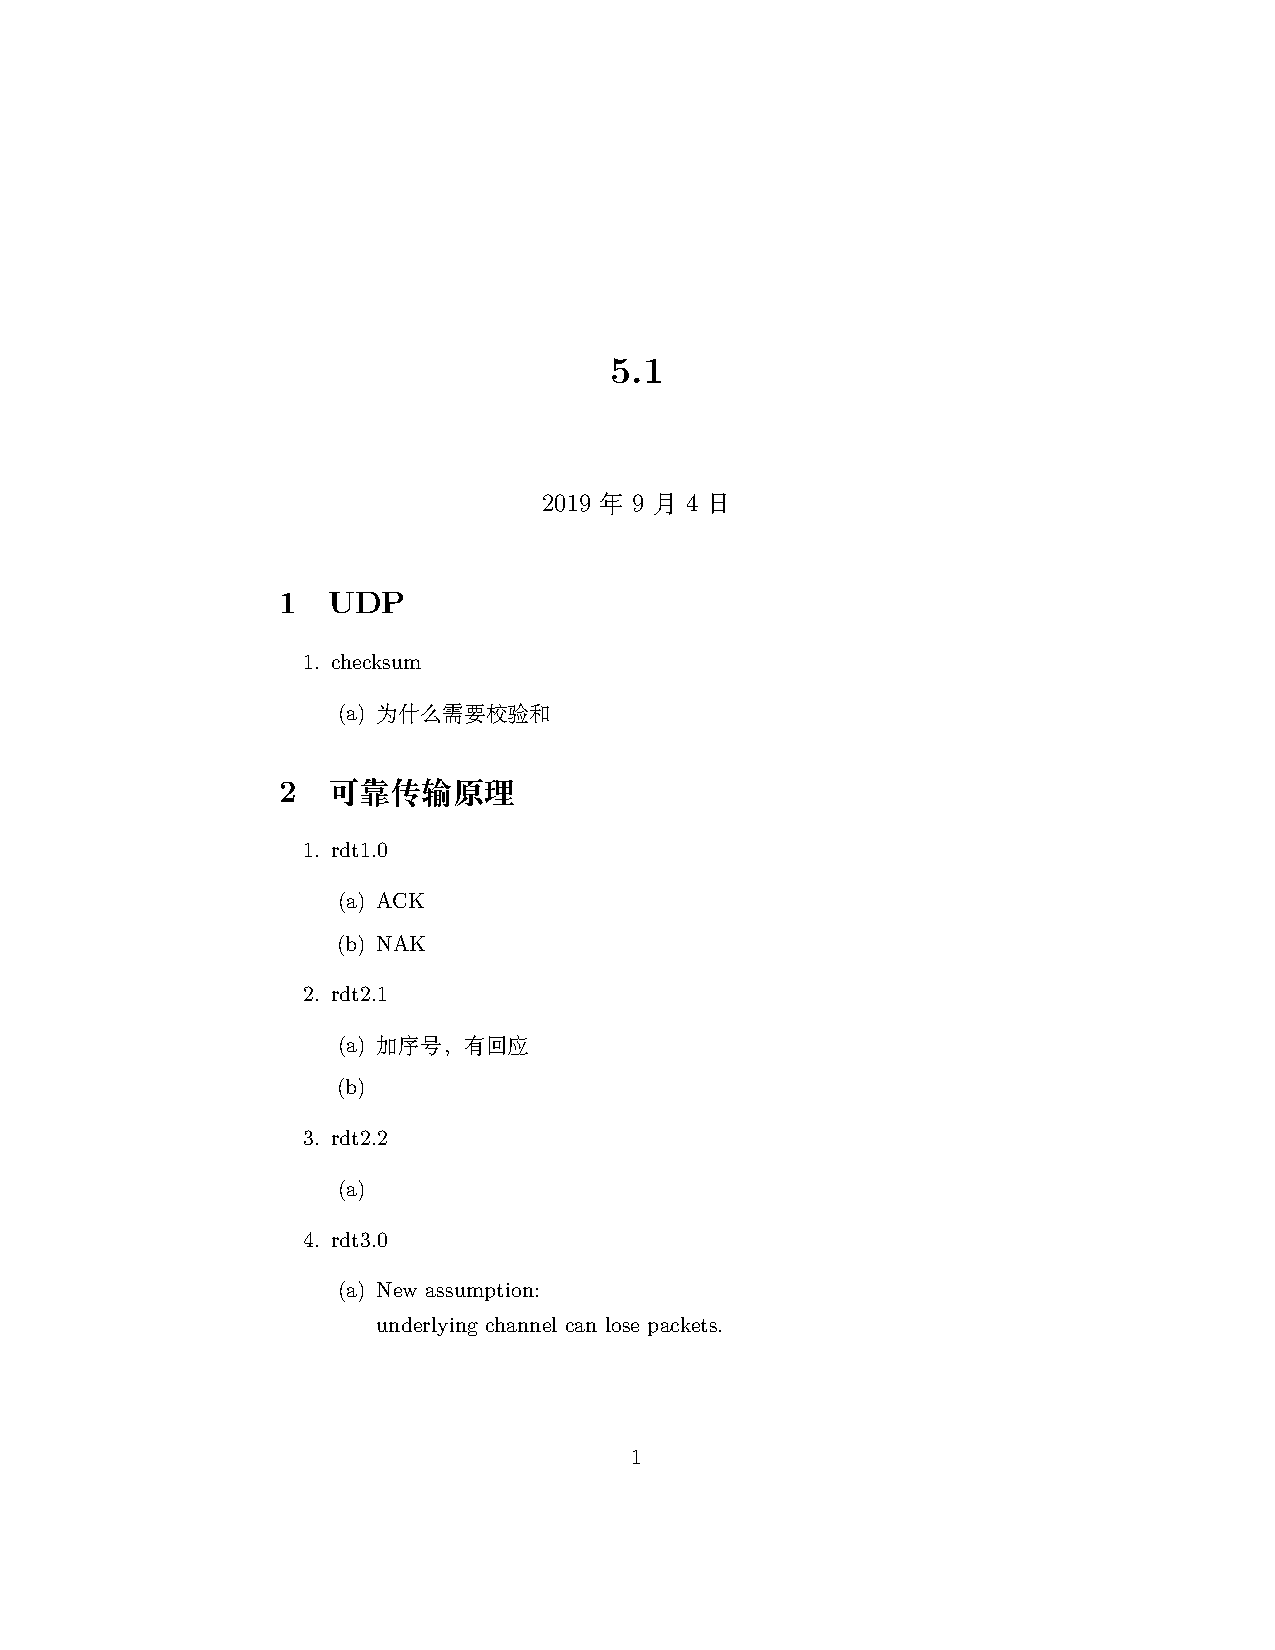
\includegraphics[width=0.8\linewidth]{picture/5-1.png} 
  
  \part{bottom-up analysis}%
  \label{prt:bottom_up_analysis}
  
  \includegraphics[width=0.8\linewidth]{picture/5-2.png} 
  
  \section{移入规约分析}%
  \label{sec:移入规约分析}
  
  \includegraphics[width=0.8\linewidth]{picture/5-3.png} 
  
  \includegraphics[width=0.8\linewidth]{picture/5-4.png} 
  
  \section{LR分析法}%
  \label{sec:lr分析法}
  
  \includegraphics[width=0.8\linewidth]{picture/5-5.png} 
  
  \includegraphics[width=0.8\linewidth]{picture/5-6.png} 
  
  \includegraphics[width=0.8\linewidth]{picture/5-7.png} 

  \includegraphics[width=0.8\linewidth]{picture/5-8.png} 

  \subsection{LR(0)分析\&\&增广文法}%
  \label{sub:分析}
  
  \includegraphics[width=0.8\linewidth]{picture/5-9.png} 
  
  \includegraphics[width=0.8\linewidth]{picture/5-10.png} 

  \includegraphics[width=0.8\linewidth]{picture/5-11.png} 

  \includegraphics[width=0.8\linewidth]{picture/5-12.png} 

  \includegraphics[width=0.8\linewidth]{picture/5-13.png} 

  \includegraphics[width=0.8\linewidth]{picture/5-14.png} 

  \includegraphics[width=0.8\linewidth]{picture/5-15.png} 

  \includegraphics[width=0.8\linewidth]{picture/5-16.png} 

  \includegraphics[width=0.8\linewidth]{picture/5-17.png} 

  \includegraphics[width=0.8\linewidth]{picture/5-18.png} 
  
  \subsection{SLR}%
  \label{sub:slr}
  
  \includegraphics[width=0.8\linewidth]{picture/5-19.png} 
  
  \subsection{LR(1)}%
  \label{sub:lr_1_}

  \includegraphics[width=0.8\linewidth]{picture/5-20.png} 

  \includegraphics[width=0.8\linewidth]{picture/5-21.png} 

  \includegraphics[width=0.8\linewidth]{picture/5-22.png} 

  \includegraphics[width=0.8\linewidth]{picture/5-23.png} 

  \includegraphics[width=0.8\linewidth]{picture/5-24.png} 
  
  
\end{document}

